\subsection{Cost Estimation Evaluation}
\label{sec:results_cost}
%
In the next experiments we evaluate our proposed cost estimation methods discussed previously in Section \ref{sec:} on the GoCard database with $SP = 5 \times 9 \times 3 = 135$.
%
Similar to previous experiments, we include the aggregate functions \texttt{count, sum, avg, min, max} and use the Earth Movers Distance (EMD) as our deviation metric for computing the utility.
%\mas{so cost was not used in the previous set of experiments?!}
%
%
We use the following query for the next experiments:
%
\begin{center}
\texttt{$Q:$ SELECT * FROM GoCard WHERE alightingstop ='University of Queensland'; }
\end{center}
%
%
%\thefontsize 
%\normalsize  
%\mas{what queries are used for input?}
We are interested in evaluating the results of the cost estimation methods based on the classical effectiveness and efficiency. 
%
For effectiveness, we asses the quality of views outputed by the proposed prioritizing algorithms $Diff DVal$, $Sela$, and $DimsHisto$ along different cost estimation methods (i.e., DB estimate and Actual Costs) comparing with SeeDB baseline.
% 
We implemented two baseline strategies: SeeDB baseline which processes the entire data and evaluates all views without any cost considerations. 
%
Thus, it provides upper bounds on latency and accuracy and a lower bound on distance error. 
%
The other baseline strategy we implemented is Actual Costs that computes the actual execution time of all views, and also the actual computational time for computing the utility of views.
%
%In addition, 

We measure the quality of results based on the accuracy and distance error. 
%
However, the efficiency of estimating methods is captured by showing the execution time across the proposed prioritizing algorithms  $Diff DVal$, $Sela$, and $DimsHisto$.
%

The first experiment evaluates the results of the Top-$25$ views using the DB Estimates (reading the costs from the database optimizer) along different space limits $R$ while comparing the estimated costs of the recommended views with the baseline.
%
As Figure \ref{fig:figCost11} shows, the accuracy of the results produced by $Sela$ , $Diff DVal$, and $DimHisto$ while reading the costs of the recommended views from the database optimizer to find a Top-$25$ views while varying $R$ is almost \%100 starting from $R = 60$.
 % \mas{if the constraint is on the number of views, then why cost is included in the priority?!!! it does not matter if a view takes a second or hour, in the end it counts as one!!}. 

While $Sela$ algorithm has the highest accuracy and the lowest error distance among all proposed algorithms as shown in Figure \ref{fig:figCost12}, the accuracy of $Diff DVal$ is very low when $R \leq 60$ because it evaluates views according to the difference of distinct values only and does not consider the query size, while $Sela$ does.
 %\mas{and why it is very low now?} 
Consequently, the error distance is higher than $Sela$ and $DimsHisto$.
%\mas{so why is it the highest now? (compared to previous experiments)} 
%
\begin{figure}[t]
  \begin{subfigure}[b]{0.32\textwidth}
    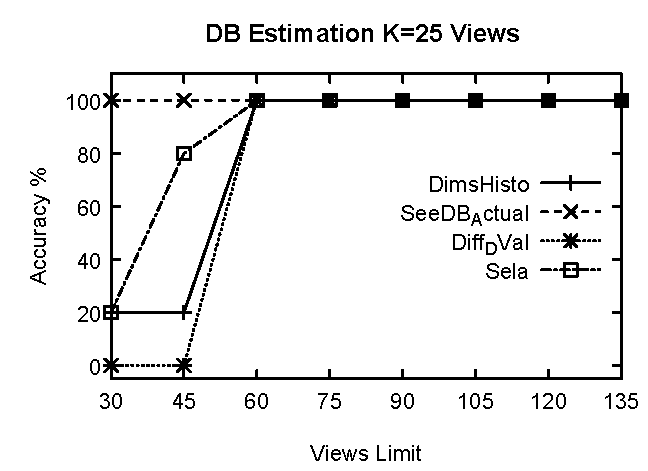
\includegraphics[width=\textwidth]{Cost11.pdf}
    \caption{Accuracy }
       \label{fig:figCost11}
  \end{subfigure}
	\begin{subfigure}[b]{0.32\textwidth}
    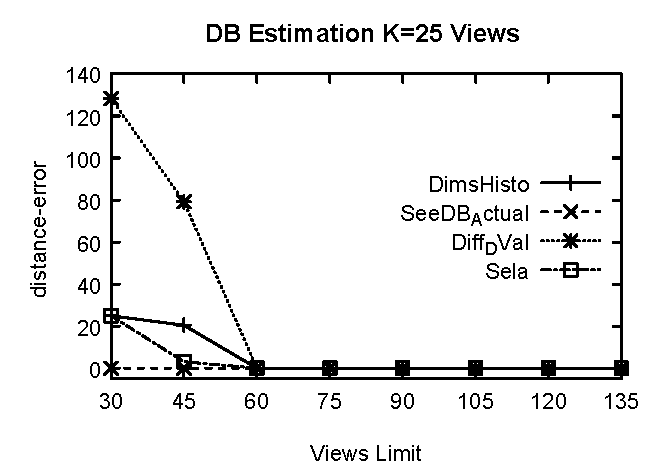
\includegraphics[width=\textwidth]{Cost12.pdf}
    \caption{Distance error}
       \label{fig:figCost12}
  \end{subfigure}
  %
  \begin{subfigure}[b]{0.32\textwidth}
    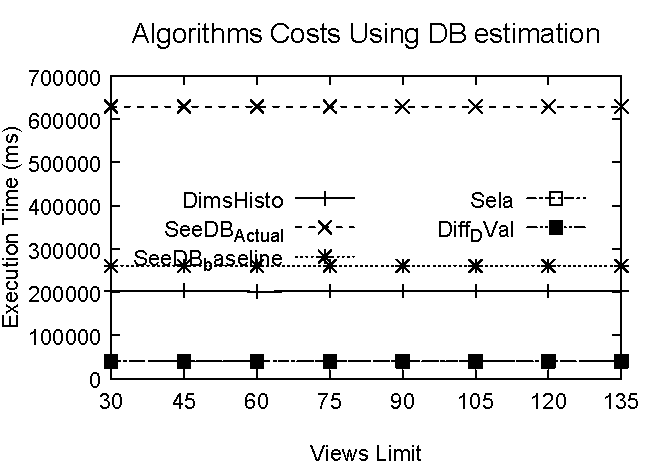
\includegraphics[width=\textwidth]{Cost21.pdf}
     \caption{Average overhead}
       \label{fig:figCost21}%
  \end{subfigure}
  \caption{Results quality and average overhead using DB Estimation}
\end{figure}
%
 %
% \begin{figure}[h]
%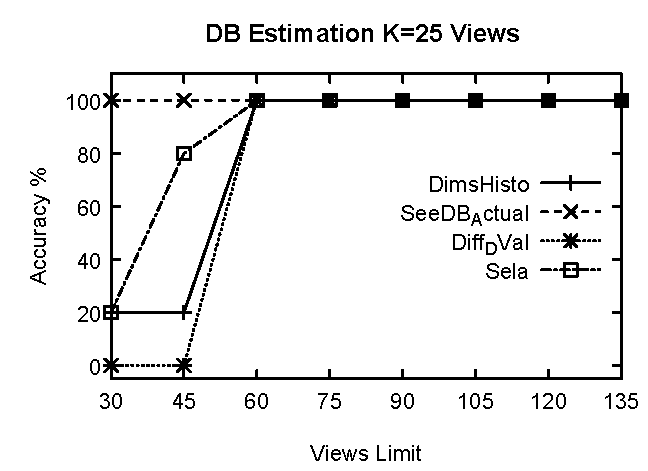
\includegraphics[width=\textwidth]{Cost11.pdf}
%\caption{Accuracy and Error Distance of algorithms $Sela$ , $N-N'$, and $DimsHisto$ across view space limits using DB Estimation}
%\label{fig:figCost11}%
%\end{figure}
%
%
%
 
The following experiment illustrates the average overhead of using different cost estimations methods along our prioritizing algorithms added to the actual SeeDB baseline.
%
In Figure \ref{fig:figCost21}, the average overhead of implementing the algorithms $Sela$ ,  $Diff DVal$, and $DimsHisto$ and reading the costs from database optimizer is shown on the y-axis.
%
As shown, computing actual costs is much expensive than running SeeDB itself.
%
This is because SeeDB does not execute all aggregate queries. 
%
For example, the average function \texttt{avg} of a view is computed by dividing the total (\texttt{sum} aggregate function) on their frequency (\texttt{count} aggregate function). 
%
Moreover, SeeDB combines the aggregate queries of the datasets $D$ and $DQ$. 
%
All algorithms have a stable performance on different space limits $R$ because the algorithms evaluate the same set of dimension attributes $A$ and outputs a subset $A'$ of top scored dimension attributes. 
%
As shown, $DimsHisto$ shows a considerable time cost since it create and assess histograms, however, both algorithms $Sela$ and $Diff DVal$ have nearly equal execution costs.
%
%\begin{figure}[t]
%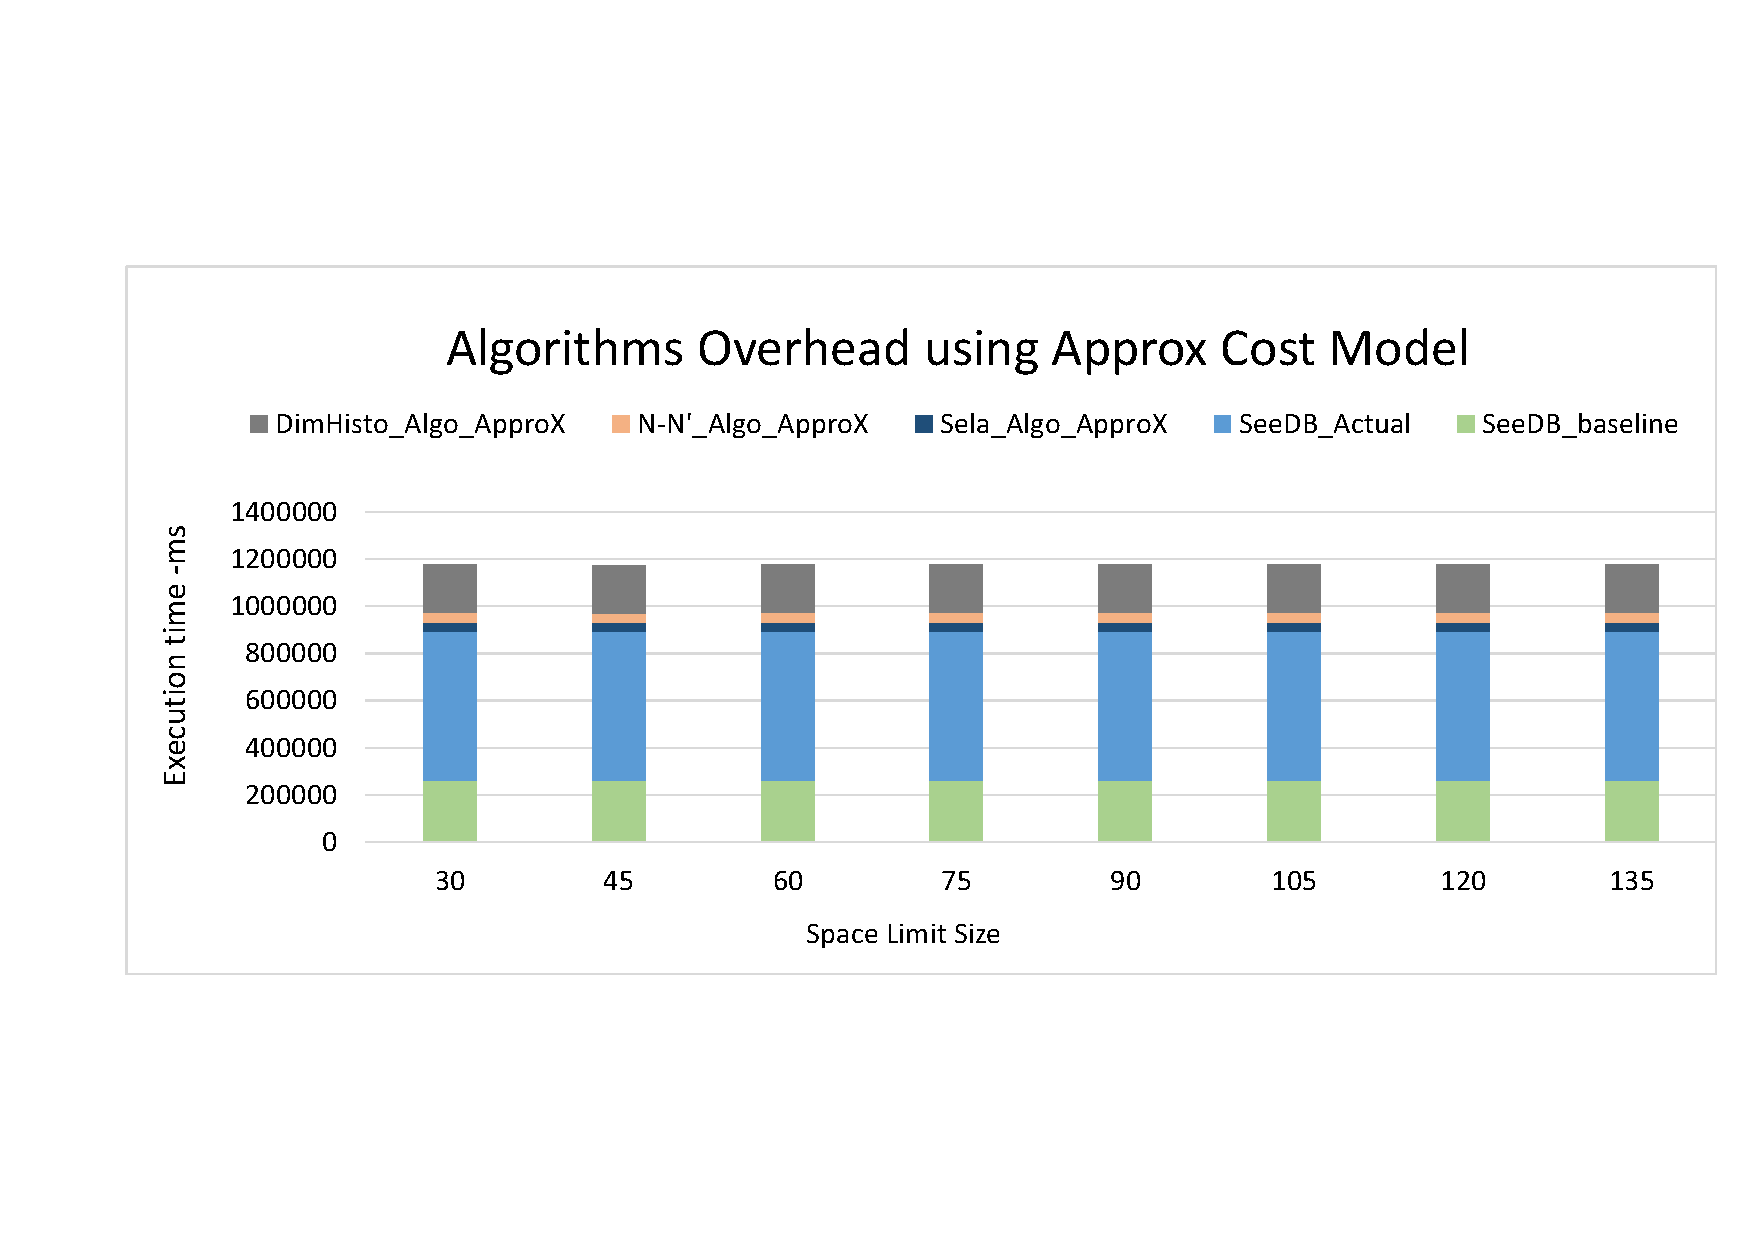
\includegraphics[width=\textwidth]{Cost22.pdf}
%\caption{The overhead of the Algorithms $Sela$ , $N-N'$, and $DimsHisto$ of using Cost Model Estimation}
%\label{fig:figCost22}%
%\end{figure}
%
 %In conclusion, the discussed algorithms $Sela$ , $Diff_DVal$, $DimsHisto$ show high 
 %accuracy and low distance errors along different space sizes while considering the costs of 
 %running and computing the deviation among the corresponding visualizations. we discussed both 
 %the results quality and the overhead of running different cost estimation techniques  
% however, our estimation approach can use any I/O cost estimation technique. %\mas{what does that mean?}. 
  